\subsection{\ref{exp:design:3} - HTTP Payload}
\label{sec:experiments:results:per-experiment:03}

In the third experiment we introduced variable application payloads. The goal of this experiment is to analyse the \gls{sm} systems when they have to process various amounts of data as application payloads. During this experiment, we generate a constant throughput of 100 requests per second, however, the application payload of each of the HTTP responses vary between 0, 1000, and 10000 bytes in size. 


\begin{figure}[!t]
    \centering
    
    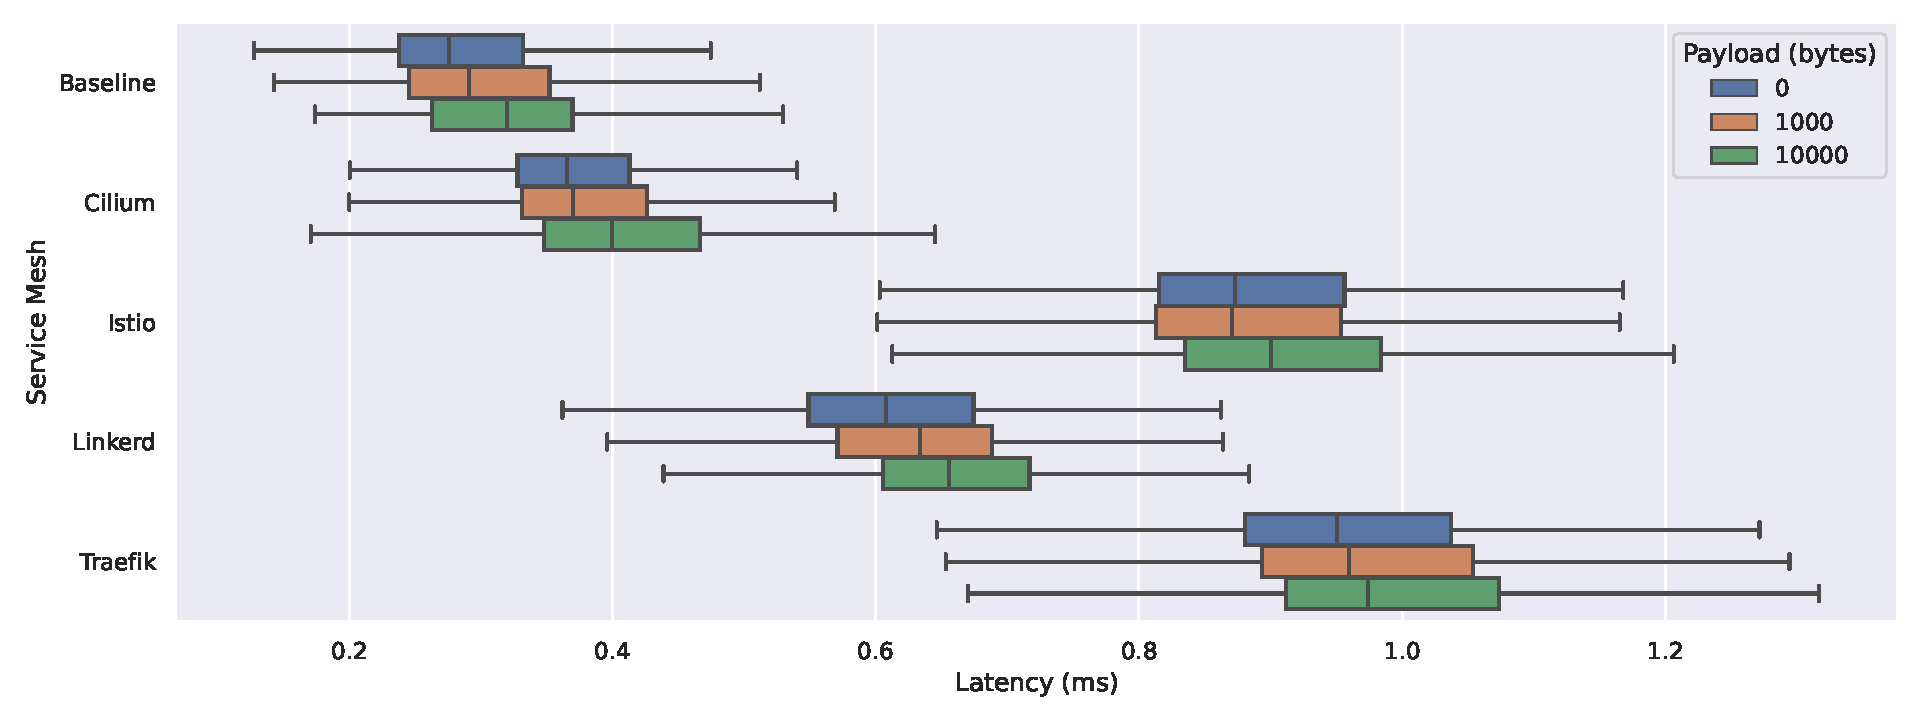
\includegraphics[width=\textwidth]{5_experimental_evaluation/figures/exp-03-latencies-all.pdf}

   \caption[Distribution of observed latencies per \gls{sm} system with varying application payload sizes]{Distribution of observed latencies per \gls{sm} system with varying application payload sizes.}
    
    \label{fig:exp:result:03:latency}
\end{figure}

In \cref{fig:exp:result:03:latency} we present the observed latency distributions of the various \gls{sm} configurations whilst processing varying levels of application payloads. On the x-axis we present the varying configurations, whilst the y-axis represents the observed latency values in milliseconds. The colours of the bars as indicated by the legend, represent the varying levels of application payload sizes encountered.

From the distributions as presented in \cref{fig:exp:result:03:latency} we can observe that the observed latencies are slightly higher of the requests that returned a larger application payload. However, the difference is very minimal, and the selected payload sizes did not seem to impact the overall observed performance. Furthermore, the application payload size also did not seem to affect the tail end latencies, as can be seen in the comparison presented in the Appendix in which we compare the 99th, 99.9th and 99.00th percentile of latencies observed (\cref{fig:exp:02:tail-latencies}).


\begin{figure}
\centering
\makebox[\linewidth][c]{
    \begin{subfigure}{.6\textwidth}
      \centering
      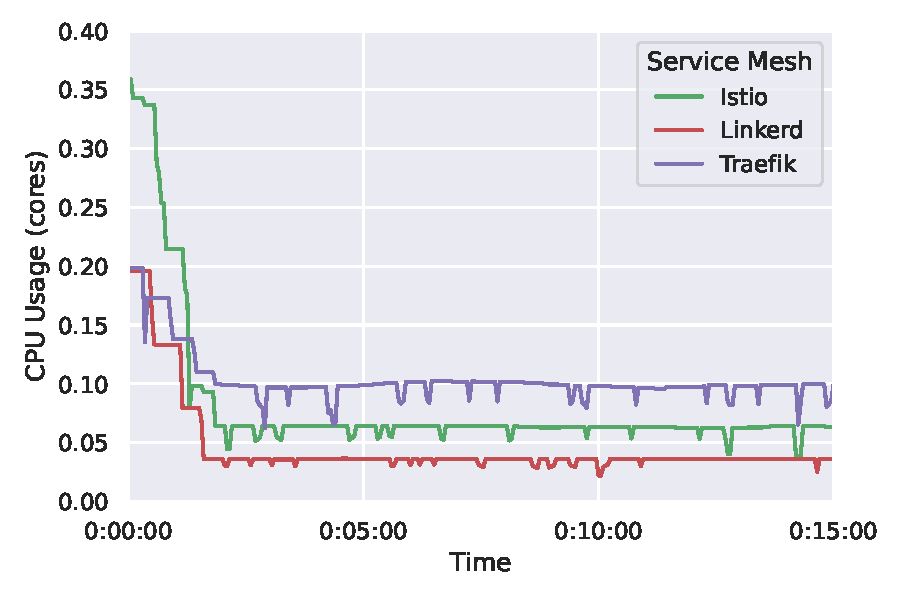
\includegraphics[width=\textwidth]{5_experimental_evaluation/figures/exp-03-cpu-utilization.pdf}
      \caption{CPU Utilization}
      \label{fig:exp:03:resource:cpu}
    \end{subfigure}
    
    
    \begin{subfigure}{.6\textwidth}
      \centering
      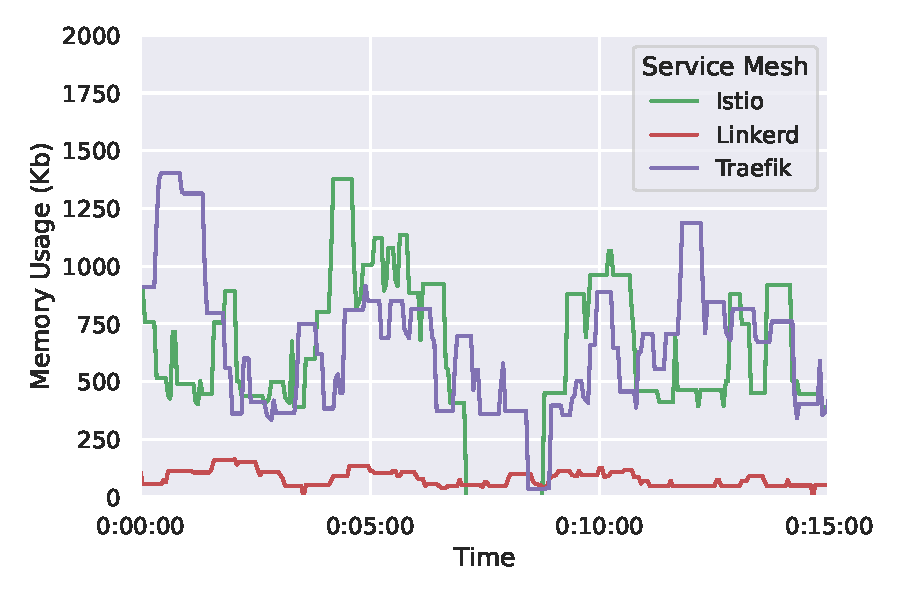
\includegraphics[width=\textwidth]{5_experimental_evaluation/figures/exp-03-memory-utilization.pdf}
      \caption{Memory Utilization}
      \label{fig:exp:03:resource:mem}
    \end{subfigure}
}
\caption[Resource utilization for \gls{sm} systems experiencing varying application payload sizes]{Resource utilization for \gls{sm} systems experiencing varying application payload sizes.}
\label{fig:exp:03:resource-utilization}
\end{figure}

In \cref{fig:exp:03:resource-utilization} we present two plots related to the resource consumption of \gls{sm} systems. These plots can be interpreted similarly, where on the y-axis we present the observed values that either represents the fraction of CPU cores used or the amount of memory consumed for a given data plane proxy. The x-axis once again represents the time delta of the experiment, which in total takes 15 minutes. The colours of the lines represent the various \gls{sm} systems which we evaluate.

We observe no significant differences for both of the plots presented in \cref{fig:exp:03:resource-utilization}. The CPU utilization is stable, aside from the initial spiked caused by the manner in which the time series data is aggregated and sampled. Furthermore, both CPU utilization and memory consumption levels for the evaluated systems conform to their expected values. This leads us to our singular conclusion from this experiment:

\begin{shaded*}
    \noindent
    \ref{exp:mf9}:
    The size of the application payload does not have a significant effect on the performance of data plane proxies and resource utilization levels.
\end{shaded*}

